\chapter{Tổng quan về điện tâm đồ}
\newpage


\section{Những khái niêm cơ bản về điện tâm đồ}
\subsection{Định nghĩa}
Điện tâm đồ (ECG) là một đường cong ghi lại các biến thiên của các điện lực do tim phát ra trong
khi hoạt động co bóp.
\begin{center}
    \begin{figure}[htp]
    \begin{center}
    %  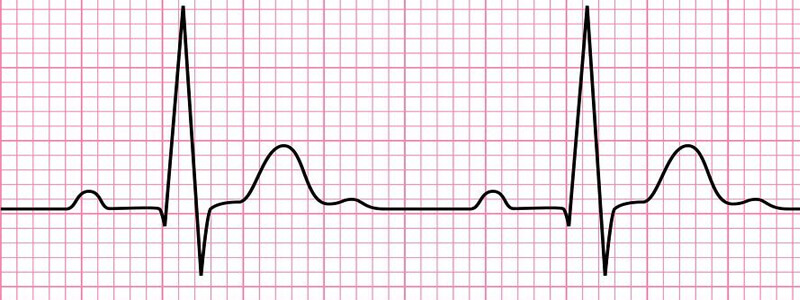
\includegraphics[scale=.]{image/week1/intro.jpg}
     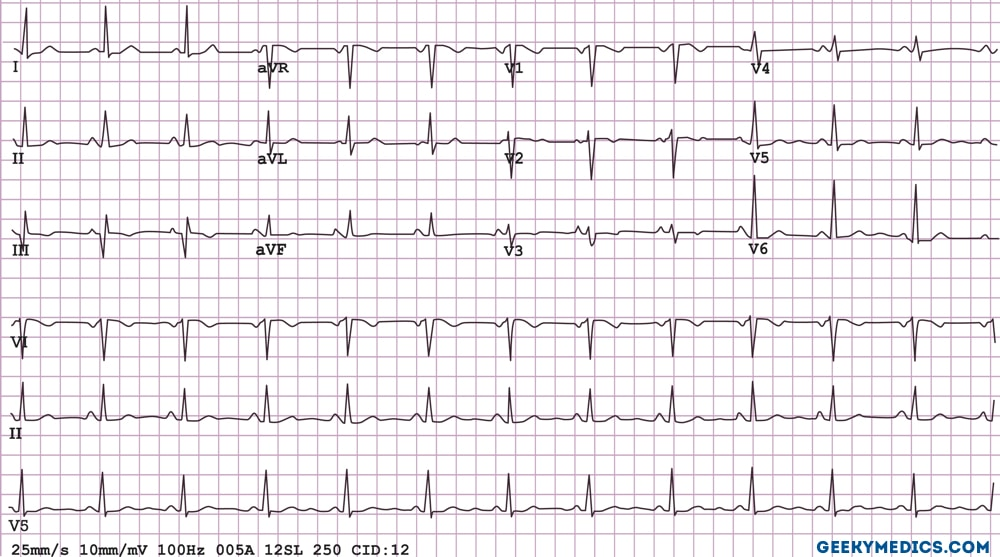
\includegraphics[scale=.4]{image/chapter1/Normal-ECG-SCALED-DOWN-WATERMARK.jpg}
    \end{center}
    \caption{Một đoạn điện tâm đồ }
    \end{figure}
\end{center}


\subsection{Hoạt động điện của cơ tim}
Do sự biến đổi hiệu thế giữa mặt trong và mặt ngoài màng tế bào cơ tim. Sự biến đổi hiệu thế này bắt nguồn từ sự di chuyển của các ion K + , Na + ,... từ ngoài vào trong tế bào và từ trong tế bào ra ngoài khi tế bào cơ tim hoạt động. Lúc này tính thẩm thấu của màng tế bào đối với các ion luôn luôn biến đổi. Do sự chênh lệch nồng độ hai bên màng tạo nên hiệu điện thế giữa hai bên màng (điện thế nghỉ).
\newpage
\begin{center}
    \begin{figure}[htp]
    \begin{center}
     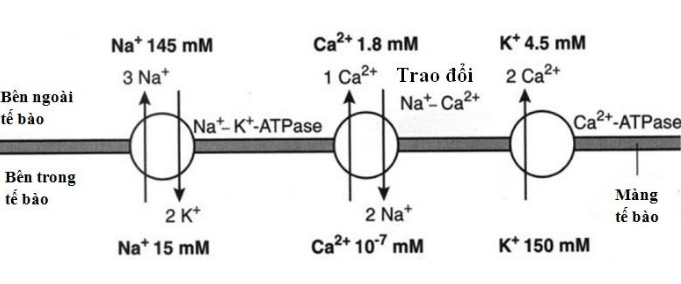
\includegraphics[scale=.4]{image/week1/h21.png}
    \end{center}
    \caption{Sự chênh lệch nồng độ của các ion Na, K, Ca \cite{huongdanDTT}}
    \end{figure}
\end{center}
\begin{center}
    \begin{figure}[htp]
    \begin{center}
     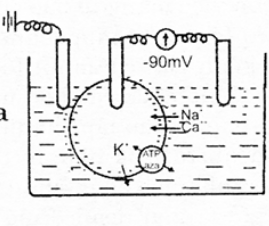
\includegraphics[scale=.6]{image/week1/h22.png}
    \end{center}
    \caption{Thí nghiệm về sự chênh lệch nồng độ của các ion Na, K, Ca \cite{huongdanDTT}}
    \end{figure}
\end{center}


\subsection{Sự hình thành điện tâm đồ}
Tim là một cơ rỗng, gồm 4 buồng dày mỏng không đều nhau. Cấu trúc phức tạp đó làm cho dòng điện hoạt động của tim (khử cực và tái cực) cũng biến thiên phức tạp hơn ở một số tế bào đơn giản. Tim hoạt động được là nhờ một xung động truyền qua hệ thống thần kinh tự động của tim. \cite{bgdtd}


\subsection{Định dạng chuẩn của một điện tâm đồ (Khổ giấy)}
Để đánh giá thời gian dài hay ngắn và biên độ cao hay thấp của các làn sóng điện tâm đồ, người ta đinh chuẩn: 
\begin{itemize}
    \item Vận tốc 25mm/s thì mỗi ô 1mm có giá trị 0,04s.
    \item Theo chiều ngang 1 ô lớn tương ứng với 1000ms.
    \item Theo chiều dọc 1 ô lớn tương ứng 500mV.
\end{itemize}
\begin{center}
    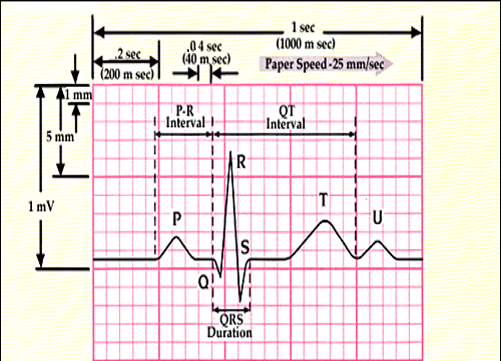
\includegraphics[scale=.6]{image/week1/new_ecg_paper.png}
    \begin{figure}[htp]
    \begin{center}
    \end{center}
    \caption{Hình ảnh một chu kỳ sóng được đo theo kích thước khổ giấy, bác sĩ căn cứ vào ô trên giấy để phát hiện bất thường ở ECG \cite{ecggiay}}
    \end{figure}
\end{center}


\subsection{Các sóng cơ bản và sự hình thành phức bộ sóng}
\begin{center}
        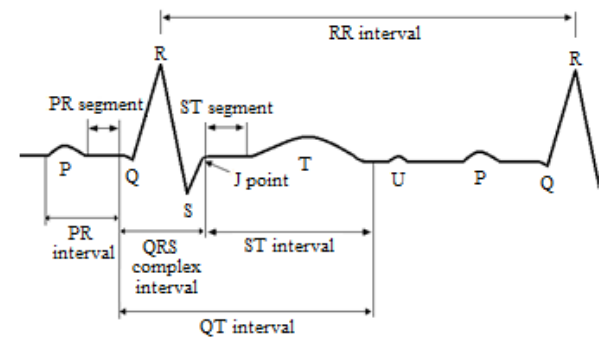
\includegraphics[scale=.4]{image/week1/h32.png}
        \begin{figure}[htp]
        \begin{center}
        \end{center}
        \caption{Tổng hợp những sóng cơ bản}
        \end{figure}
    \end{center}
\begin{itemize}
    \item Những sóng cơ bản trong ECG là:
    \begin{itemize}
        \item Nhĩ đồ
        \begin{itemize}
            \item Sóng P: một làn sóng dương thấp, nhỏ, tầy đầu.
        \end{itemize}
        \item Thất đồ
        \begin{itemize}
            \item Phức bộ sóng QRS (QRS complex): gồm ba làn sóng cao, nhọn Q, R, S biến thiên phức tạp.(Sóng dương đầu tiên là sóng R, sóng âm trước sóng Q, sóng âm đầu tiên sau sóng R là sóng S, nếu không có sóng R thì là sóng QS).
            \item Sóng T: một sóng dương thấp, tầy đầu.
            \item Sóng U: một sống chậm nhỏ xuất hiện vào giai đoạn muộn, sau sóng T.
        \end{itemize}        
    \end{itemize}
    \item Tóm lại:
    \begin{itemize}
        \item Điện tâm đồ bình thường của mỗi nhát bóp tim (hay chu chuyển tim) gồm 6 làn
        sóng nối tiếp nhau mà người ta dùng 6 chữ cái liên tiếp để đặt tên là P, Q, R, S, T, U. Trong đó,
        người ta phân ra một nhĩ đồ, sóng P, một thất đồ: các sóng Q, R, S, T, U với thời gian truyền đạt
        nhĩ thất: khoảng PQ.(Người ta không đo thời gian của T vì nó rất thay đổi, tùy từng người. Hơn nữa, chỗ khởi điểm của nó tiếp với ST rất thoai thoải, khó đo).
    \end{itemize}
\end{itemize}

\subsection{Các chuyển đạo thông dụng}

\subsubsection{Điện trường tim:}
Cơ thể con người là một môi trường dẫn điện; vì thế, dòng điện do tim phát ra được dẫn truyền khắp cơ thể, ra tới da, biến cơ thể thành một điện trường của tim. Nếu ta đặt hai điện cực lên bất cứ hai điểm nào đó có điện thế khác nhau của điện trường đó, ta sẽ thu được một dòng điện thể hiện hiệu thế giữa hai điểm đó và gọi là một chuyển đạo hay đạo trình (lead). Nó hiện ra trên máy ghi bằng một đường cong điện tâm đồ có một hình dạng nào đó tùy theo địa điểm đặt các điện cực. Đường thẳng nối hai địa điểm đặt điện cực trên cơ thể gọi là trục chuyển đạo.

\subsubsection{Chuyển đạo mẩu:}
\begin{center}
    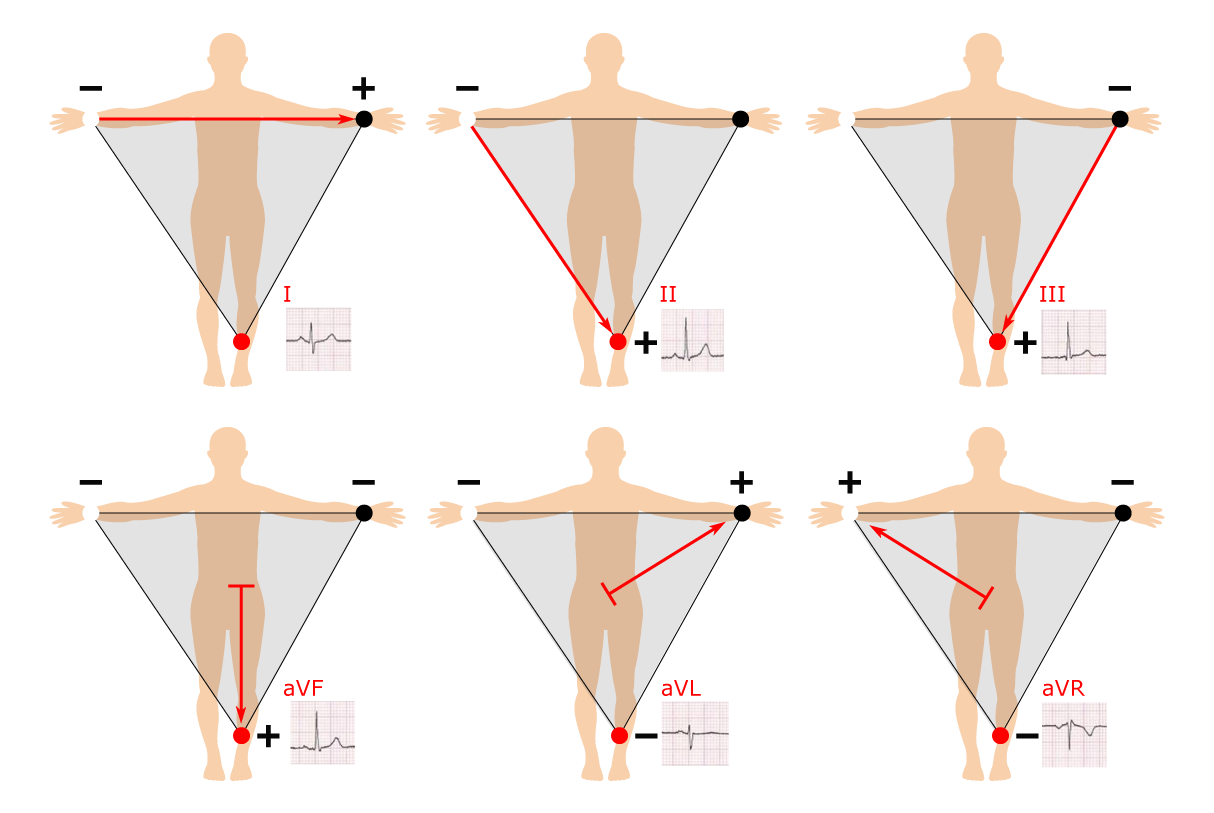
\includegraphics[scale=.25]{image/week1/chuyendaochi.png}
    \begin{figure}[htp]
    \begin{center}
    \end{center}
    \caption{Chuyển đạo chi \cite{chuyendao}}
    \end{figure}
\end{center}
Tất cả 6 chuyển đạo: D1, D2, D3, aVR, aVL, aVF được gọi chung là các chuyển đạo ngoại biên vì đều có điện cực thăm dò đặt ở các chi. Chúng hỗ trợ cho nhau “dò xét” các rối loạn của dòng điện tim thể hiện ở bốn phía xung quanh quả tim trên mặt phẳng chắn (frontal plane).

\subsubsection{Chuyển đạo trước tim:}
\begin{center}
    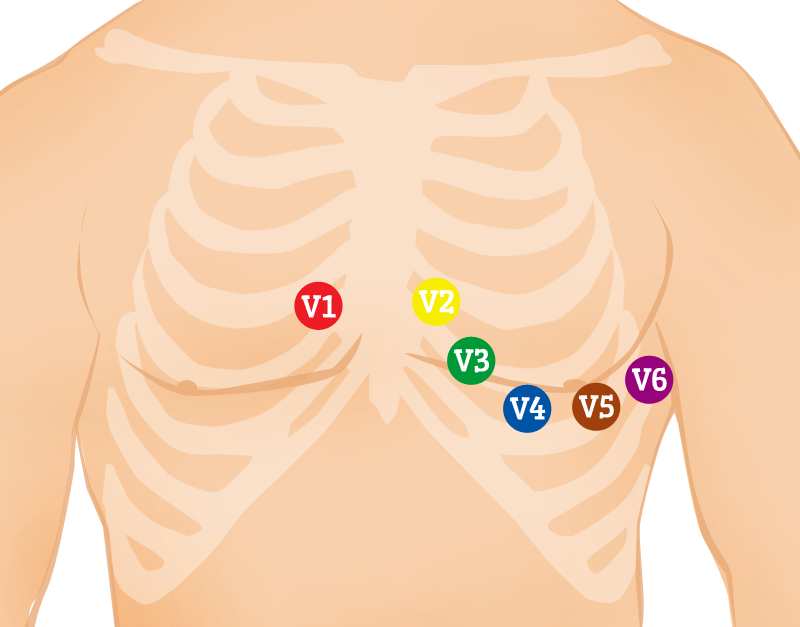
\includegraphics[scale=.3]{image/week1/chuyendaotruocnguc.png}
    \begin{figure}[htp]
    \begin{center}
    \end{center}
    \caption{Chuyển đạo trước tim \cite{chuyendao}}
    \end{figure}
\end{center}
Người ta thường ghi đồng loạt cho bệnh nhân 6 chuyển đạo trước tim thông dụng nhất, kí hiệu bằng chữ V (voltage) kèm theo các chỉ số từ 1 đến 6.(V1, V2,…,V6).

\subsubsection{Một số chuyển đạo khác:}
V7, V8, V9(điện cực ở mé trái và sau lồng ngực dùng để thăm dò thất trái), V3R, V4R, V5R, V6R(điện cực ở mé phải lồng ngực dùng để nghiên cứu thất phải hay tim sang phải), chuyển đạo thực quản (Kí hiệu VOE), chuyển đạo trong buồng tim, điện đồ His.

\subsection{Vị trí gắn các điện cực và tư thế bệnh nhân khi đo 12 chuyển đạo}
\begin{center}
    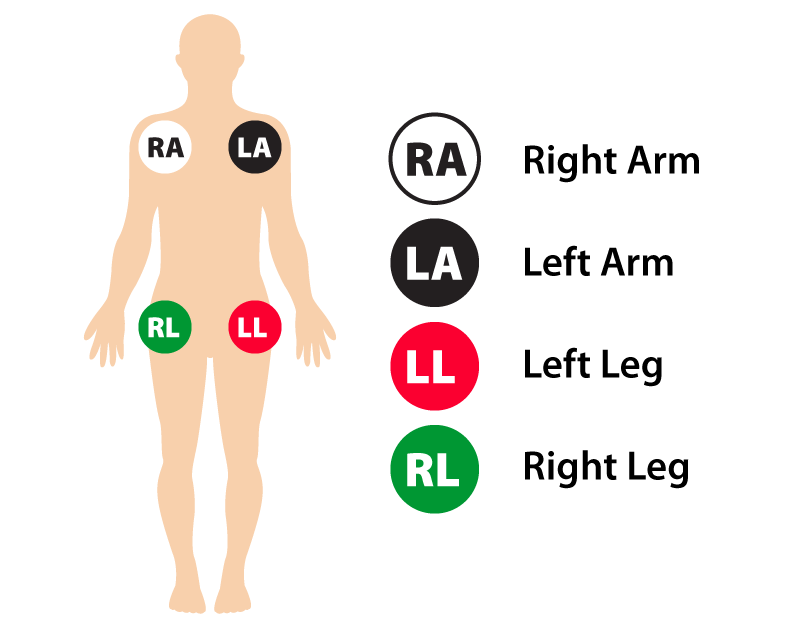
\includegraphics[scale=.3]{image/week1/datdiencuc.png}
    \begin{figure}[htp]
    \begin{center}
    \end{center}
    \caption{Các vị trí đặt điện cực \cite{chuyendao}}
    \end{figure}
\end{center}
\begin{center}
    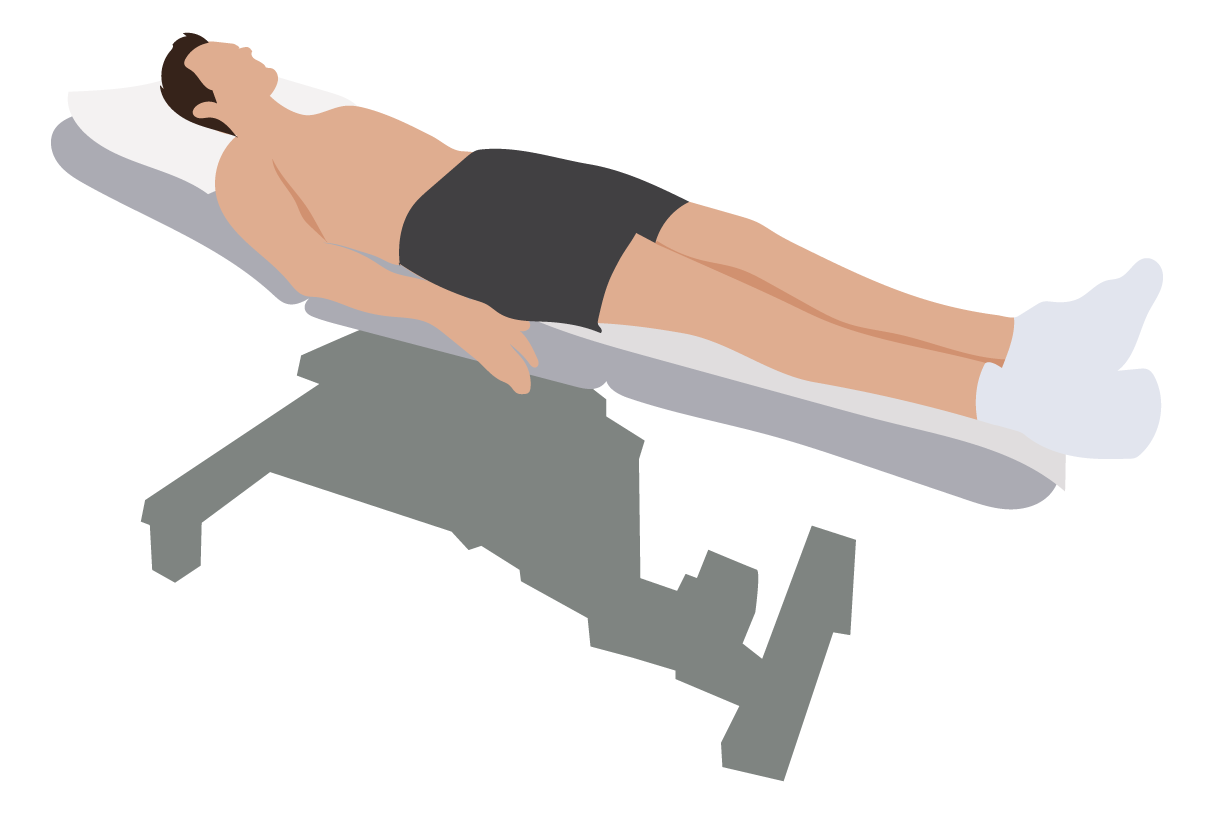
\includegraphics[scale=.25]{image/week1/benhnhannam.png}
    \begin{figure}[htp]
    \begin{center}
    \end{center}
    \caption{Tư thế  nằm của bệnh nhân khi ghi điện tim \cite{chuyendao}}
    \end{figure}
\end{center}


\section{Đọc một điện tâm đồ}
\subsection{Những bước phân tích trước khi đọc một điện tâm đồ}
Điện tâm đồ (ECG) là một đường cong ghi lại các biến thiên của các điện lực do tim phát ra trong khi hoạt động co bóp.\cite{huongdanDTT}

\begin{enumerate}
    \item Trước khi đọc điện tâm đồ, phải nắm vững tuổi, giới tính, chẩn đoán lâm sàng của bệnh
    nhân. Ngoài ra, còn nên biết thêm sơ lược bệnh án, hình ảnh X quang, các kết quả xét nghiệm khác và nhất là hai vấn đề sau đây:
    \begin{itemize}
        \item Khổ người bệnh nhân gầy béo, cao thấp ảnh hưởng rất nhiều đến tư thế tìm và biên độ sóng, nó ảnh hưởng nhiều đến chẩn đoán dày thất.
        \item Có đang dùng thuốc trợ tim hay thuốc chống loạn nhịp dài ngày không? Nhất là digitan và quinidin… vì các thuốc này tác động rất nhiều đến hình dạng điện tâm đồ và dễ làm sai lạc chẩn đoán cơ bản.
    \end{itemize}
    \item Kiểm tra kỹ thuật ghi điện tâm đồ, phát hiện ghi sai, ảnh hưởng tạp, milivôn lấy đúng 1cm
    hay không? Tốc độ ghi bao nhiêu? Nghĩa là các đường kẻ dọc cách nhau bao nhiêu phần trăm
    giây
    \item Nhịp tim: bước vào đọc điện tâm đồ trước hết bao giờ cũng phải xem nhịp xoang hay
    không xoang? Có những rối loạn nhịp tim gì? Đừng bao giờ quên tính tần số tim. Nếu có blốc
    nhĩ-thất thì phải tính riêng cả tần số nhĩ.
    \item Trục điện tim với góc alpha, tư thế tim.
    \item Hình dạng các sóng: đọc đồng thời ở cả 12 chuyển đạo thông dụng:
    \begin{itemize}
        \item Sóng P: chiều cao (biên độ), chiều rộng (thời gian), hình dạng (âm, dương, hai pha, móc).
        \item Khoảng PQ dài bao nhiêu?
        \item Phức bộ QRS: biên độ và thời gian chung và riêng của sóng Q, hình dạng (móc…).
        \item Riêng với V1 và V5 thì tìm thêm thời gian xuất hiện nhánh nội điện.
        \item Đoạn ST có chênh không?
        \item Sóng T (và sóng U): dạng (dương, âm hay hai pha), biên độ.
        \item Khoảng QT dài bao nhiêu?
    \end{itemize}
    \item Kết luận chẩn đoán: về tổn thương cơ tim và về rối loạn nhịp tim.
\end{enumerate}

\subsection{Phát hiện sai lầm trong ghi điện tâm đồ}
\subsubsection{Ghi điện tâm đồ sai lầm}
\begin{enumerate}
    \item Mắc dây sai tay: thí dụ mắc nhầm dây điện cực đỏ sang tay trái và dây điện cực vàng sang tay phải: như vậy trên điện tâm đồ, ta sẽ thấy các sóng ở D1 đều âm (nhất là P1 âm), D2 có dạng D3 và ngược lại, aVR có dạng aVL và ngược lại. Còn các chuyển đạo trước tim thì không ảnh hưởng gì và điều này giúp ta phân biệt tật bẩm sinh “tim sang phải”.
    \item Vặn nút máy ghi nhầm thứ tự các chuyển đạo.
    \item Đánh dấu và viết tên nhầm chuyển đạo này với chuyển đạo kia.
    \item Dán nhầm thứ tự các chuyển đạo hoặc dán nhầm điện tâm đồ của người này sang người khác, khi dán băng điện tâm đồ vào tờ hồ sơ điện tâm đồ của từng bệnh nhân.
\end{enumerate}
Muốn phát hiện các lầm lẫn này, trước hết phải luôn luôn nhớ thuộc lòng hình dạng bình thường của 12 chuyển đạo thông dụng. Hơn nữa, cần chú ý mấy qui luật cơ bản sau:
\begin{enumerate}
    \item Định luật Einthoven: do cách bố trí các trục của 3 chuyển đạo mẫu, Einthoven đã tính ra được công thức sau D1 + D3 = D2. Thí dụ: sóng R1 (sóng R ở D1) là 10mm, R3 là 8mm thì R2 phải là 18mm. Nếu đo thấy không đúng như thế thì có thể là ghi sai. Nhưng lẽ tất nhiên, đó là kể những ca sai nhiều, còn nếu chỉ sai lệch vài ba milimét thì không kể vì có thể là do ảnh hưởng của sự thở hay độ lệch điện trở tổ chức.
    \item Tính chất liên tục của các chuyển đạo trước tim: do các chuyển đạo đó có điện cực thăm dò đặt liên tiếp cạnh nhau nên các sóng của chúng cũng phải biến thiên liên tục. Thí dụ: sóng R thấp nhất ở V1, sau đó cao dần lên qua V2, V3, V4 đến V5 rồi hơi thấp xuống ở V6. Nếu ở một ca ta thấy R ở V2 cao vọt lên hay thấp hẳn xuống, đi lệch hẳn khỏi đường cong biểu diễn trên mà không nằm trong một bảng bệnh cảnh điện tâm đồ bệnh lí nào rõ ràng thì chắc là ghi sai. Đối với sóng T cũng có quy luật tương tự (xem mục sóng T).
    \item Tính chất giống nhau của một số chuyển đạo: các chuyển đạo D1, aVL, V5, V6 có trục chuyển đạo gần nhau và cùng hướng nên hay có hình dạng các sóng hao hao giống nhau. D3 và aVF cũng vậy. Thí dụ khi thấy có một sóng Q ở D1 thì thường cũng phải thấy có một sóng Q tương tự ở V5, V6. Nếu không có thì có thể là ghi sai. Tuy nhiên, điều đó không tuyệt đối vì còn phải tính đến các rối loạn bệnh lí làm biến đổi các chuyển đạo một cách không đều nhau nữa.
\end{enumerate}
